\newSec[Regelerarten]{Arten von Reglergliedern}{2}

In diesem Kapitel sollen grundlegende Bausteine der Regelungtechnik beschrieben werden. Diesbezüglich erhebt dieses Kapitel keinen Anspruch auf Vollständigkeit. Auf eine detallierte Beschreibung, welche \ua\ das Zeitverhalten betrachten, soll hier außen vor gelassen werden.
Als weitere Einschränkung soll sich die Betrachtung der Bausteine ausschließlich auf zeitdiskrete Systeme beziehen.


\newSec[ControlP]{P-Glied}{3}
Die Abkürzung \texttt{P} in der Bezeichnung \textit{P-Glied} steht für \textit{proportional}. Hierbei wird eine die Eingangsgröße um einen Faktor $k_P$ verstärkt. \comp{RT1} %Seite 220

\begin{equ}[!ht]
\begin{equation}
y_k = k_P * x_k
\end{equation}
\caption{Übertragungsfunktion des P-Glieds}
\end{equ}


\begin{figure}[ht!]
\vspace{0.25cm}
\begin{center}
\fbox{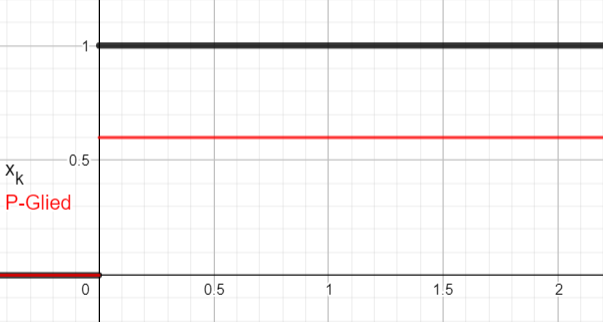
\includegraphics[width=8cm]{Pictures/StepP.png}}
\caption{Sprungantwort eines P-Glieds}
\label{fig:StepP}
\end{center}

\vspace{0.25cm}
\refImgShort{fig:StepPID} zeigt charakteristischen Sprungantwort des \textit{P-Glieds}. Hier wurde der Parameter $k_P$ mit dem Wert 0,6 gewählt, um die Sichtbarkeit in der Abbildung zu erhöhen.
\end{figure}

In einem geschlossenen Regelkreis führt der Einsatz eines \textit{P-Glieds} ohne weitere Regelbausteine zu einer bleibenden Regelabweichung.
Aus den Zusammenhängen $e=w-r$ und $r=e*k_P$\footnote{Für diesen Ansatz werden sämtliche Bausteine nach \textit{E} (\textit{Regelglied}) (siehe \refImg{fig:Contr}) ignoriert. Daraus folgt: $r = m$.} lässt sich die dauerhafte Regelabweichung in Abhängigkeit des Verstärkungsfaktors bestimmen: $e=\frac{w}{1-k_P}$.

Entgegen steht der Vorteil eine schnellen und dauerhaften Reaktion auf eine Regeldifferenz.

\FloatBarrier
\newSec[ControlI]{I-Gield}{3}
Wie sich aus dem Namen des \textit{Integral-Glieds} ableiten lässt, bildet dieser Baustein ein Integral über dem Eingangssignal.
Hierdurch können physikalische Umrechnungen oder Prozesse abgebildet werden. Als Beispiele kann an dieser Stelle der Füllstand eines Tanks oder die Ermittlung einer Geschwindigkeit aus Beschleunigungsdaten genannt werden. \comp{RT1}

\begin{equ}[!ht]
\begin{equation}
y_k = y_{k-1} + k_I * x_k*{\Delta t}
\end{equation}
\caption{Übertragungsfunktion des I-Glieds}
\end{equ}

\begin{figure}[ht!]
\vspace{0.25cm}
\begin{center}
\fbox{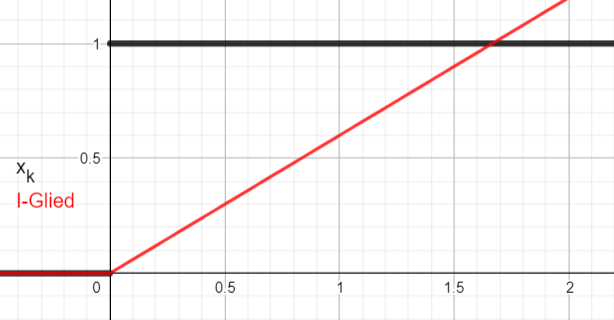
\includegraphics[width=8cm]{Pictures/StepI.png}}
\caption{Sprungantwort eines I-Glieds}
\label{fig:StepI}
\end{center}

\vspace{0.25cm}
\end{figure}

Da das \textit{I-Glied} Regeldifferenzen aufsummiert, läuft die Regeldifferenz im geschlossenen Regelkreis asymptotisch gegen den Wert 0.


\FloatBarrier
\newSec[ControlD]{D-Gield}{3}
In der betrachteten Literatur spielen D-Glieder keine signifikante Rolle. \compB{RT1}{SV1}
Dennoch sollen sie hier als Grundlage für \textit{PID}-Glieder beschrieben werden.

Bei einem \textit{D-Glied} handelt es sich um ein differentielles Glied. Somit lässt sich hiermit die Veränderung des Eingangssignals ermitteln.\comp{ContrD}\missing[Diese Quelle iO?]

Das Ausgangssignal des \textit{D-Glieds} kann durch folgende Formel berechnet werden, welche sich aus der Diskretisierung der Differenztationsfunktion ergibt.

\begin{equ}[!ht]
\begin{equation}
y_k = k_D * \frac{x_k - x_{k-1}}{\Delta t}
\end{equation}
\caption{Übertragungsfunktion des D-Glieds}
\end{equ}

\begin{figure}[ht!]
\vspace{0.25cm}
\begin{center}
\fbox{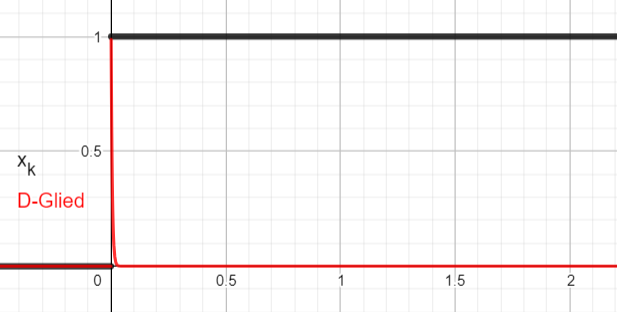
\includegraphics[width=8cm]{Pictures/StepD.png}}
\caption{Sprungantwort eines D-Glieds}
\label{fig:StepD}
\end{center}

\vspace{0.25cm}
\refImgShort{fig:StepD} zeigt die Sprungantwort eines \textit{D-Glieds}. Diese ist ist ein Ausschlag, welcher für den Zeitschritt anhält, in dem sich die ansteigende Flanke des Sprungs befindet.
\end{figure}

Durch den Einfluss eines \textit{D-Glieds} kann auf schnelle Änderungen einer Größe reagiert werden. Die Regeldifferenz der Sprungantwort ist nach dem anfänglichen Ausschlag mit dem Wert 1 (100\%) anzunehmen.


\FloatBarrier
\newSec[ControlPID]{PID-Regler}{3}
Das \textit{PID-Glied} bildet die Vereinigung der vorab genannten Regelbausteine. Als Ausgangssignal wird die Summe über die einzelnen Regelbausteine gebildet:
\begin{equ}[!ht]
\begin{equation}
y_k = y_{k(P)} + y_{k(I)} + y_{k(D)}
\end{equation}
\caption{Übertragungsfunktion des PID-Glieds}
\end{equ}

\begin{figure}[ht!]
\vspace{0.25cm}
\begin{center}
\fbox{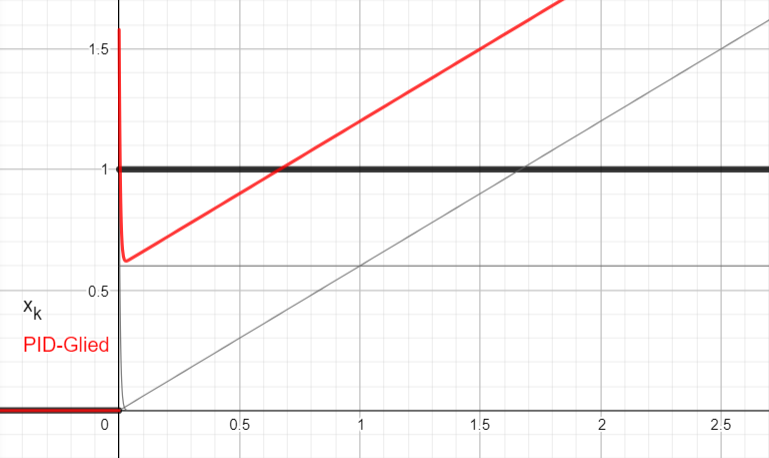
\includegraphics[width=8cm]{Pictures/StepPID.png}}
\caption{Sprungantwort eines PID-Glieds}
\label{fig:StepPID}
\end{center}

\vspace{0.25cm}
\refImgShort{fig:StepPID} zeigt die Sprungantwort eines \textit{PID-Glieds}. Hierbei setzt sich das Signal als Summe des P-, des I- und des D-Glieds zusammen, welche in grau angedeutet sind.
\end{figure}

Das \textit{PID-Glied} vereinigt die Vorteile der Einzelbausteine. Die genannten Nachteile werden durch eines der anderen Regelglieder ausgehebelt.\\
Daher wird das \textit{PID-Glied} als universal-Regelbaustein eingesetzt, wobei geeignete Verstärkungsfaktoren ausgewählt und optimiert werden müssen.


\FloatBarrier
\newSec[ControlPT]{PT-Glied}{3}
Um reale Systeme abzubilden, kann das \textit{PT-Glied} eingesetz werden. Als Beispiele können hier die Temperatur in einem Gas ein eingebrachter Energie oder die Drehzahl eines Motors (massebehaftet) genannt werden.\\
Die Einbindung des \textit{PT-Glieds} erfolgt die Vor- \bzw\ Nachschaltung an Berechnung der idealisierten Größe.


\begin{equ}[!ht]
\begin{equation}
y_k = y_{k-1} + (k_{PT1}*x_k - y_{k-1}) * \frac{\Delta t}{T_1}
\end{equation}
\caption{Übertragungsfunktion des PT-Glieds}
\end{equ}


\begin{figure}[ht!]
\vspace{0.25cm}
\begin{center}
\fbox{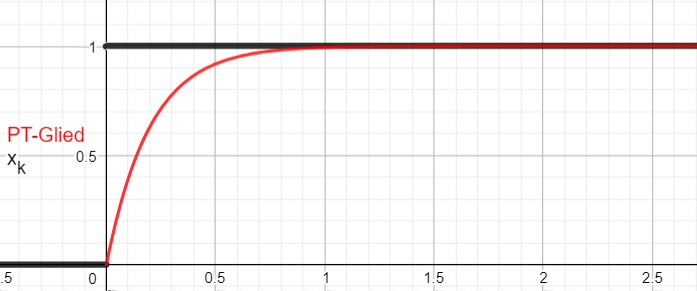
\includegraphics[width=8cm]{Pictures/StepPT.png}}
\caption{Sprungantwort eines PT-Glieds}
\label{fig:StepPT}
\end{center}

\vspace{0.25cm}
\end{figure}




\newSec[ControlPT]{Tt-Glied}{3}
Bei einem \textit{Totzeit-Glied} handelt es sich um Baustein, welcher vorwiegend zur Abbildung realer Systeme genutzt wird. Als Beispiel kann hier die Füllmenge eines Förderbands genannt werden, wobei der Füllstandssensor nach der Befülleinrichtung angeordnet werden muss.\\
Totzeiten erhöhen die Instabilität von Systemen. \missing[Quelle??]

Da dieser Baustein nur zur Vollständigkeit genannt werden soll, wird von einer Vertiefung der Thematik an dieser Stelle abgesehen.


















